% !TEX program = xelatex
% /root, 2026-10-21: condensed notes from preserved notes 01--06 and Tutorials.
\documentclass[11pt,a4paper]{article}
% Adapted from templates/latex/报告模板.zip (XeLaTeX, unofficial CUHK-SZ report style).
\usepackage{fontspec,xeCJK}
\setmainfont{texgyretermes}[Extension=.otf,UprightFont=*-regular,BoldFont=*-bold,ItalicFont=*-italic,BoldItalicFont=*-bolditalic]
\setsansfont{texgyreheros}[Extension=.otf,UprightFont=*-regular,BoldFont=*-bold,ItalicFont=*-italic,BoldItalicFont=*-bolditalic]
\setmonofont{Menlo}[Scale=0.84]
\setCJKmainfont{Songti SC}[AutoFakeBold=2]
\setCJKsansfont{Hiragino Sans GB}
\setCJKmonofont{Hiragino Sans GB}
\usepackage{microtype}
\usepackage[a4paper,margin=25mm,headheight=22pt,headsep=8mm,footskip=12mm]{geometry}
\usepackage{graphicx,amsmath,amssymb,mathtools}
\usepackage{booktabs,longtable,tabularx,array,calc}
\usepackage{enumitem,listings,fvextra,caption,fancyhdr,lastpage,titlesec,xcolor}
\usepackage{etoolbox,float,adjustbox,pdflscape,needspace,soul,newunicodechar,seqsplit}
\usepackage{tikz}
\usetikzlibrary{arrows.meta,positioning,calc,fit,shapes.geometric,shapes.multipart,matrix}
\usepackage[unicode,pdfencoding=auto,bookmarksnumbered=false]{hyperref}
\definecolor{CUHKPurple}{HTML}{5C2267}
\definecolor{CUHKGold}{HTML}{C99A2E}
\definecolor{Ink}{HTML}{20242B}
\definecolor{Muted}{HTML}{626B75}
\definecolor{Rule}{HTML}{D8DCE0}
\definecolor{CodeBg}{HTML}{F5F6F8}
\color{Ink}
\hypersetup{colorlinks=true,linkcolor=CUHKPurple,urlcolor=CUHKPurple,pdfauthor={CSC5041 Personal Study Materials},pdftitle={CSC5041 Revision Materials}}
\setlist{leftmargin=*,itemsep=2pt,topsep=4pt}
\setlength{\parindent}{0pt}
\setlength{\parskip}{5pt}
\setlength{\emergencystretch}{3em}
\linespread{1.08}
\setcounter{secnumdepth}{0}
\setcounter{tocdepth}{2}
\titleformat{\section}{\sffamily\LARGE\bfseries\color{CUHKPurple}}{}{0pt}{}
\titleformat{\subsection}{\sffamily\large\bfseries\color{CUHKPurple}}{}{0pt}{}
\titleformat{\subsubsection}{\sffamily\normalsize\bfseries\color{Ink}}{}{0pt}{}
\titlespacing*{\section}{0pt}{1em}{0.65em}
\titlespacing*{\subsection}{0pt}{1em}{0.4em}
\titlespacing*{\subsubsection}{0pt}{0.7em}{0.25em}
\captionsetup{font=small,labelfont={bf,color=CUHKPurple},labelsep=period}
\pagestyle{fancy}\fancyhf{}
\fancyhead[L]{\sffamily\small\color{Muted}CSC5041 · Database Systems}
\fancyhead[R]{\sffamily\small\color{Muted}\VolumeShort}
\fancyfoot[L]{\sffamily\scriptsize\color{Muted}The Chinese University of Hong Kong, Shenzhen}
\fancyfoot[R]{\sffamily\scriptsize\color{Muted}\thepage\ / \pageref*{LastPage}}
\renewcommand{\headrulewidth}{0.4pt}
\newcommand{\VolumeShort}{Weeks 1--5}
\fancypagestyle{cover}{\fancyhf{}\fancyfoot[R]{\sffamily\small 2026-10-20}\renewcommand{\headrulewidth}{0pt}}
\newcommand{\StudyCover}[3]{%
 \thispagestyle{cover}
 \noindent\begin{minipage}[c]{0.12\textwidth}
\includegraphics[width=0.82\linewidth]{assets/CUHK_Logo.png}\end{minipage}%
 \begin{minipage}[c]{0.85\textwidth}{\sffamily\bfseries\large The Chinese University of Hong Kong, Shenzhen}\par{\sffamily\small\color{Muted}Personal study materials · Unofficial}\end{minipage}
 \par\vspace{12pt}{\color{CUHKGold}\rule{\linewidth}{1.2pt}}\par\vspace{20mm}
 {\sffamily\bfseries\Huge\color{CUHKPurple}#1}\par\vspace{9mm}
 {\sffamily\LARGE #2}\par\vspace{5mm}{\large\color{Muted}#3}\par
 \vfill{\small Adapted from the supplied academic report template.\par Original teaching materials remain unchanged.\par LaTeX edition: 20 October 2026.}\clearpage}
\lstdefinestyle{studysql}{language=SQL,basicstyle=\ttfamily\small,keywordstyle=\color{CUHKPurple}\bfseries,stringstyle=\color{CUHKGold!65!black},commentstyle=\color{Muted},backgroundcolor=\color{CodeBg},frame=single,rulecolor=\color{Rule},breaklines=true,breakatwhitespace=false,columns=fullflexible,keepspaces=true,showstringspaces=false,tabsize=4,aboveskip=8pt,belowskip=8pt}
\lstset{style=studysql}
\DefineVerbatimEnvironment{StudyCode}{Verbatim}{breaklines=true,breakanywhere=true,fontsize=\small,frame=single,rulecolor=\color{Rule},framesep=6pt,baselinestretch=1.1}
\newcommand{\tightlist}{\setlength{\itemsep}{0pt}\setlength{\parskip}{0pt}}
\newcommand{\passthrough}[1]{#1}
\newcommand{\pandocbounded}[1]{\begin{adjustbox}{max width=\linewidth,max totalheight=.78\textheight,keepaspectratio}#1\end{adjustbox}}
\newcommand{\StudyFormula}[1]{\par\noindent\begin{adjustbox}{max width=\linewidth}\(\displaystyle #1\)\end{adjustbox}\par}
\newcommand{\StudyVisual}[2]{\begin{figure}[H]\centering\StudyDiagram{#1}{#2}\end{figure}}
\newcommand{\StudyLandscapeER}{\clearpage\begin{landscape}\thispagestyle{empty}\begin{center}{\sffamily\large\bfseries\color{CUHKPurple}Tutorial 1: complete ER diagram}\par\vspace{4mm}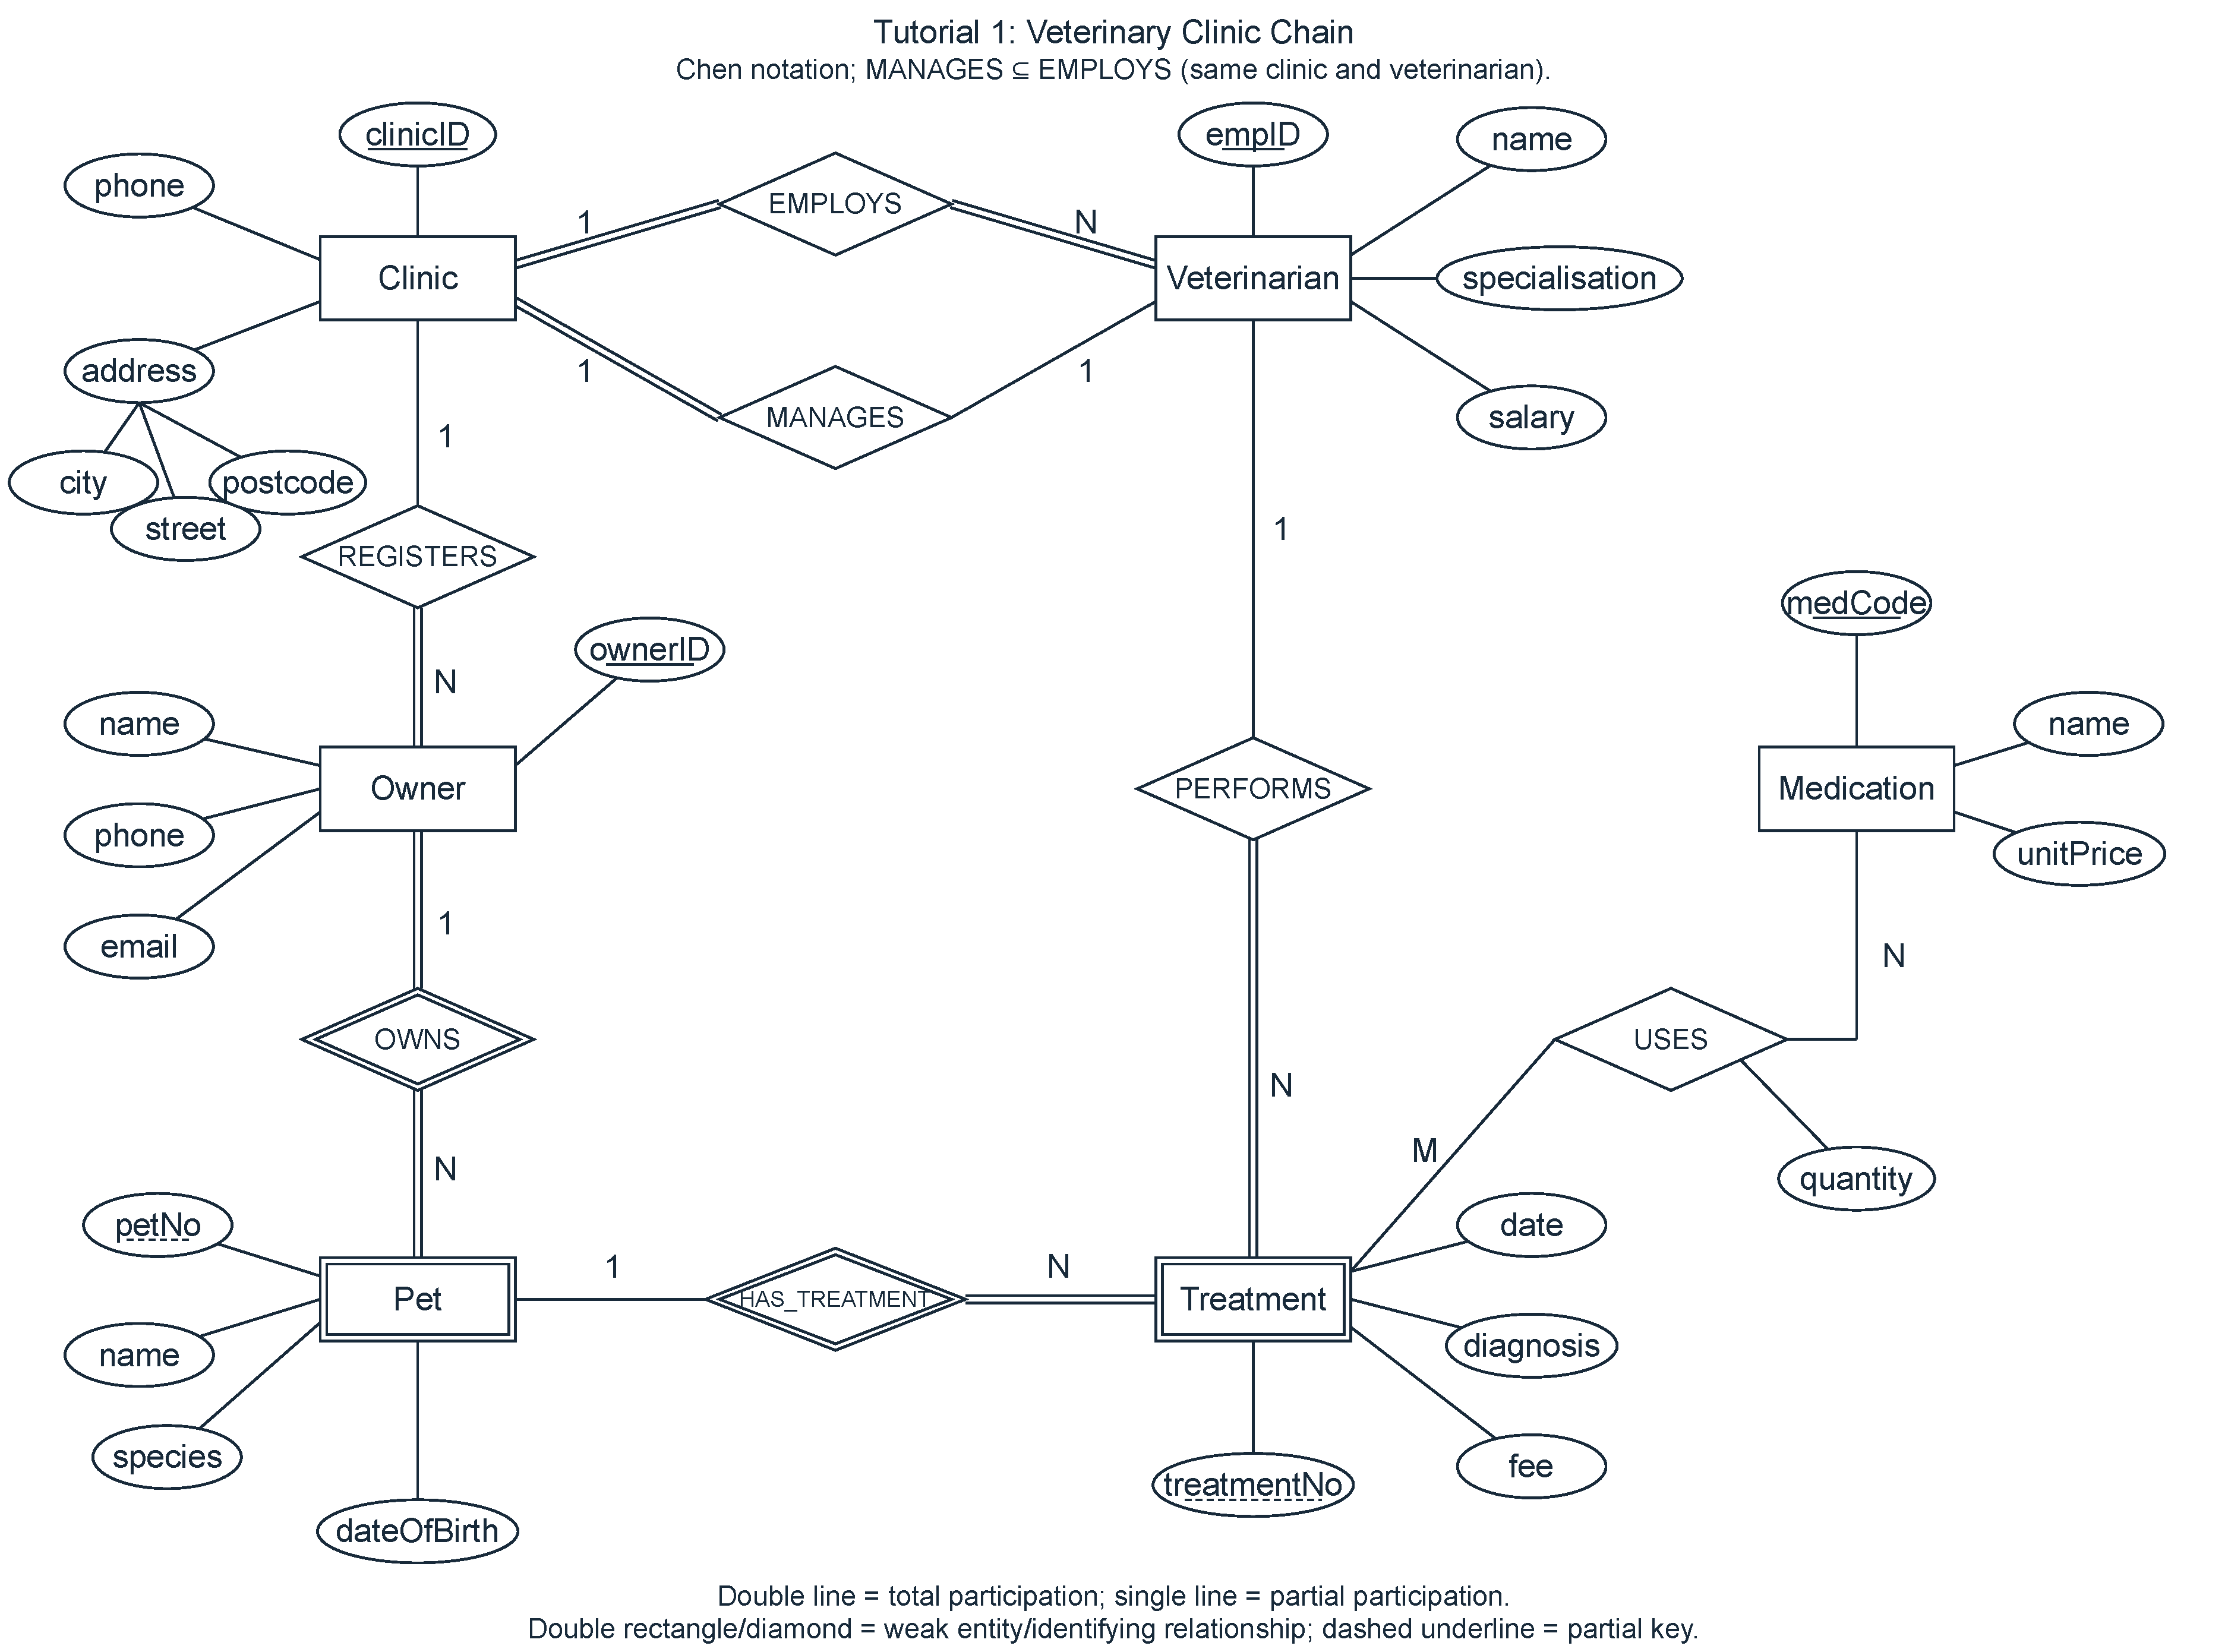
\includegraphics[width=\linewidth,height=.86\textheight,keepaspectratio]{figures/tutorial1_er.pdf}\end{center}\end{landscape}\clearpage}
\setlength{\tabcolsep}{4pt}
\renewcommand{\arraystretch}{1.17}
\AtBeginEnvironment{longtable}{\small}
\setlength{\LTleft}{0pt}\setlength{\LTright}{0pt}
\newunicodechar{σ}{\ensuremath{\sigma}}
\newunicodechar{π}{\ensuremath{\pi}}
\newunicodechar{ρ}{\ensuremath{\rho}}
\newunicodechar{γ}{\ensuremath{\gamma}}
\newunicodechar{θ}{\ensuremath{\theta}}
\newunicodechar{⋈}{\ensuremath{\bowtie}}
\newunicodechar{÷}{\ensuremath{\div}}
\newunicodechar{∀}{\ensuremath{\forall}}
\newunicodechar{∃}{\ensuremath{\exists}}
\newunicodechar{∈}{\ensuremath{\in}}
\newunicodechar{∉}{\ensuremath{\notin}}
\newunicodechar{⊆}{\ensuremath{\subseteq}}
\newunicodechar{∪}{\ensuremath{\cup}}
\newunicodechar{∩}{\ensuremath{\cap}}
\newunicodechar{∧}{\ensuremath{\land}}
\newunicodechar{∨}{\ensuremath{\lor}}
\newunicodechar{¬}{\ensuremath{\neg}}
\newunicodechar{≠}{\ensuremath{\ne}}
\newunicodechar{∅}{\ensuremath{\varnothing}}
\newunicodechar{≤}{\ensuremath{\le}}
\newunicodechar{≥}{\ensuremath{\ge}}
\newunicodechar{×}{\ensuremath{\times}}
\newunicodechar{→}{\ensuremath{\rightarrow}}
\newunicodechar{←}{\ensuremath{\leftarrow}}
\newunicodechar{⇒}{\ensuremath{\Longrightarrow}}
\newunicodechar{−}{\ensuremath{-}}
\newunicodechar{✓}{\ensuremath{\checkmark}}
\newunicodechar{☐}{\ensuremath{\square}}
\newunicodechar{☑}{\ensuremath{\boxtimes}}
% Editable teaching diagrams. Examples reuse Chapters 01--06; no measured data.
% Requires tikz, amsmath, amssymb; colors are defined by the document preamble.
\newcommand{\SDtext}[2]{\ifx\SDlang\SDzh #1\else #2\fi}
\newcommand{\StudyDiagram}[2]{\begingroup
  \edef\SDlang{#2}\def\SDzh{zh}%
  \tikzset{sd box/.style={draw=CUHKPurple,rounded corners=3pt,fill=CUHKPurple!4,align=center,inner sep=7pt,font=\fontsize{10}{13}\selectfont},sd arrow/.style={-{Stealth[length=2mm]},thick,draw=CUHKPurple},sd note/.style={align=center,text=Muted,font=\fontsize{9}{12}\selectfont},sd table/.style={draw=Rule,fill=CodeBg,inner sep=6pt,align=center,font=\fontsize{10}{13}\selectfont}}%
  \csname SDdiagram#1\endcsname
\endgroup}

\newcommand{\SDdiagramschemas}{%
\begin{tikzpicture}[node distance=9mm]
\node[sd box,text width=11.8cm] (e) {\SDtext{外模式：不同用户的视图}{External schemas: different user views}\\\texttt{Student view}\quad|\quad\texttt{Registrar view}};
\node[sd box,text width=11.8cm,below=of e] (c) {\SDtext{概念模式：整个数据库的逻辑结构}{Conceptual schema: database-wide logical structure}\\\texttt{Student(sid,name,major), Course(...), Enrolment(...)}};
\node[sd box,text width=11.8cm,below=of c] (i) {\SDtext{内模式：文件、页、索引与存储组织}{Internal schema: files, pages, indexes and storage organization}};
\draw[sd arrow] (e)--(c);\draw[sd arrow] (c)--(i);
\node[sd note,below=8mm of i,text width=12.6cm] {\SDtext{逻辑独立性：改变概念模式，保持外模式及应用不变。\\物理独立性：改变内模式，保持概念模式不变。}{Logical independence: change conceptual schema; preserve external schemas/applications.\\Physical independence: change internal schema; preserve conceptual schema.}};
\end{tikzpicture}}

\newcommand{\SDdiagramdbms}{%
\begin{tikzpicture}[node distance=7mm]
\node[sd box,text width=11cm] (a) {\SDtext{用户／应用程序}{User / application}\quad\texttt{SELECT ...}};
\node[sd box,text width=11cm,below=of a] (q) {\SDtext{查询处理器：解析、优化、执行}{Query processor: parse, optimize, execute}};
\node[sd box,text width=11cm,below=of q] (s) {\SDtext{存储管理器：缓冲区、文件与索引访问}{Storage manager: buffers, files and index access}};
\node[sd box,text width=11cm,below=of s] (d) {\SDtext{数据库文件＋系统目录（元数据）}{Database files + system catalog (metadata)}};
\draw[sd arrow] (a)--(q);\draw[sd arrow] (q)--(s);\draw[sd arrow] (s)--(d);
\node[sd note,text width=12cm,below=7mm of d] {\SDtext{简化的概念流程；权限、完整性、并发与恢复机制贯穿请求处理。}{Simplified conceptual flow; authorization, integrity, concurrency and recovery support request handling.}};
\end{tikzpicture}}

\newcommand{\SDdiagramweak}{%
\begin{tikzpicture}[node distance=10mm]
\node[sd box,text width=11.4cm] (b) {\textbf{Building}\quad\SDtext{完整键}{Full key}: $\{buildingID\}$};
\node[sd box,text width=11.4cm,below=of b] (r) {\textbf{Room}\quad\SDtext{局部键}{Partial key}: $\{roomNo\}$\\\SDtext{完整键}{Full key}: $\{buildingID,roomNo\}$};
\node[sd box,text width=11.4cm,below=of r] (d) {\textbf{Desk}\quad\SDtext{局部键}{Partial key}: $\{deskNo\}$\\\SDtext{完整键}{Full key}: $\{buildingID,roomNo,deskNo\}$};
\draw[sd arrow] (b)-- node[right,sd note]{\SDtext{继承所有者的完整键}{Carry owner's full key}} (r);
\draw[sd arrow] (r)-- node[right,sd note]{\SDtext{继承所有者的完整键}{Carry owner's full key}} (d);
\node[sd note,text width=12.6cm,below=7mm of d] {\SDtext{自编示例。房号只在楼内唯一，桌号只在房间内唯一。\\Desk 的外键为 $(buildingID,roomNo)$，不能只保留 $roomNo$。}{Original example. Room numbers are local to a building; desk numbers are local to a room.\\Desk references Room with $(buildingID,roomNo)$, not $roomNo$ alone.}};
\end{tikzpicture}}

\newcommand{\SDdiagramintegrity}{%
\begin{tikzpicture}
\node[sd table] (s) at (0,0) {\textbf{Student}\\\begin{tabular}{cc}\underline{sid}&name\\\hline S01&Amy\\S02&Ben\end{tabular}};
\node[sd table] (e) at (7.3,0) {\textbf{Enrolment}\\\begin{tabular}{cc}\underline{sid}&\underline{cid}\\\hline S01&C01\\S01&C02\end{tabular}};
\draw[sd arrow] (e.west)-- node[above,sd note]{\texttt{FK: sid $\to$ sid}} (s.east);
\node[sd note,text width=4.6cm] at (0,-2.15) {\SDtext{主键：唯一且非空}{Primary key: unique and non-NULL}\\$PK(Student)=\{sid\}$};
\node[sd note,text width=6cm] at (7.3,-2.15) {\SDtext{复合主键：整组唯一；sid 可以重复}{Composite PK: pair unique; sid may repeat}\\$PK(Enrolment)=\{sid,cid\}$};
\node[sd box,text width=11.7cm] at (3.6,-4.1) {$\pi_{sid}(Enrolment)\subseteq\pi_{sid}(Student)$\\\SDtext{本例 sid 属于主键，故非空；一般外键是否可空取决于约束。}{Here sid is part of the PK, so non-NULL; a general FK's nullability depends on constraints.}};
\node[sd note,text width=12cm] at (3.6,-5.7) {\SDtext{自编示例；仅展示 sid 引用。cid 还需引用 Course 的键。}{Original example; only the sid reference is shown. cid must also reference Course's key.}};
\end{tikzpicture}}

\newcommand{\SDdiagrammapping}{%
\begin{tikzpicture}
\node[sd box,text width=11.8cm] (a) at (0,0) {\textbf{1:N}\quad\texttt{Department}\ $1\;\text{---}\;N$\ \texttt{Employee}\\\texttt{Department(\underline{deptID}, name)}\\\texttt{Employee(\underline{empID}, name, deptID)}};
\node[sd note,text width=12cm] at (0,-1.65) {$Employee.deptID\longrightarrow Department.deptID$\\\SDtext{外键放 N 侧；若 Employee 全参与，再加 NOT NULL。}{Place FK on the N side; add NOT NULL if Employee participation is total.}};
\node[sd box,text width=11.8cm] (b) at (0,-3.45) {\textbf{M:N}\quad\texttt{Student}\ $M\;\text{---}\;N$\ \texttt{Course}\\\texttt{Enrolment(\underline{sid}, \underline{cid})}\quad $PK=\{sid,cid\}$};
\node[sd note,text width=12cm] at (0,-5) {$Enrolment.sid\to Student.sid\qquad Enrolment.cid\to Course.cid$\\\SDtext{建立关联关系；关系属性也放在此处。外键本身不保证两端全参与。}{Create an association relation; put relationship attributes here. FKs alone do not ensure total participation.}};
\node[sd note,text width=12cm] at (0,-6.1) {\SDtext{自编简化示例；假设同一学生与课程最多关联一次。}{Original simplified example; assume at most one association per student--course pair.}};
\end{tikzpicture}}

\newcommand{\SDdiagramoperators}{%
\begin{tikzpicture}
\node[sd table] (c) at (0,0) {\textbf{Course}\\\begin{tabular}{ccc}cid&dept&credits\\\hline C1&CS&4\\C2&CS&3\\C3&Math&4\end{tabular}};
\node[sd table] (s) at (7.6,1.3) {\begin{tabular}{ccc}cid&dept&credits\\\hline C1&CS&4\end{tabular}};
\node[sd table] (p) at (7.6,-1.4) {\begin{tabular}{c}dept\\\hline CS\\Math\end{tabular}};
\draw[sd arrow] (c.north east)--node[above,sloped,sd note]{$\sigma_{dept='CS'\,\land\,credits>3}$}(s.west);
\draw[sd arrow] (c.south east)--node[below,sloped,sd note]{$\pi_{dept}$}(p.west);
\node[sd note,text width=12cm] at (3.6,-3) {\SDtext{选择：筛行，保留所有列。投影：选列，并消除重复。\\采用第 05 章数据；为图示省略 title 列。}{Selection: filter rows, keep all columns. Projection: retain columns and eliminate duplicates.\\Chapter 05 data; the title column is omitted for display.}};
\end{tikzpicture}}

\newcommand{\SDdiagramdivision}{%
\begin{tikzpicture}
\node[sd table] at (0,0) {\textbf{Takes}\quad$R(sid,cid)$\\\begin{tabular}{cc}sid&cid\\\hline S1&C1\\S1&C2\\S2&C1\\S2&C3\\S3&C3\end{tabular}};
\node[sd table] at (4.25,0.6) {\textbf{Target}\quad$S(cid)$\\\begin{tabular}{c}cid\\\hline C1\\C2\end{tabular}};
\node[sd table] at (9,0.6) {\SDtext{结果}{Result}\quad$R\div S$\\\begin{tabular}{c}sid\\\hline S1\end{tabular}};
\draw[sd arrow] (5.95,0.6)--node[above,sd note]{$\forall cid\in S$}(7.4,0.6);
\node[sd box,text width=11.8cm] at (4.4,-2.6) {$R\div S=\{s\in\pi_{sid}(R)\mid\forall c\in S,\ (s,c)\in R\}$\\\SDtext{覆盖每一门目标课程；允许额外课程；重复不能弥补缺项。}{Cover every target course; extra courses are allowed; duplicates cannot fill a gap.}};
\node[sd note,text width=12cm] at (4.4,-4) {\SDtext{沿用第 05 章数据。S2 缺 C2；S3 缺 C1、C2。\\候选来自 $\pi_{sid}(R)$，因此 S4 不在除法的候选域内。}{Chapter 05 data. S2 lacks C2; S3 lacks C1 and C2.\\Candidates come from $\pi_{sid}(R)$, so S4 is outside this division's candidate domain.}};
\end{tikzpicture}}

\newcommand{\SDdiagramsqlflow}{%
\begin{tikzpicture}[node distance=5mm]
\node[sd box,text width=10.6cm] (f) {\texttt{FROM / JOIN}\quad\SDtext{形成输入行}{Form input rows}};
\node[sd box,text width=10.6cm,below=of f] (w) {\texttt{WHERE}\quad\SDtext{筛选行：只保留 TRUE}{Filter rows: retain TRUE only}};
\node[sd box,text width=10.6cm,below=of w] (g) {\texttt{GROUP BY / aggregation}\quad\SDtext{形成组并聚合}{Form groups and aggregate}};
\node[sd box,text width=10.6cm,below=of g] (h) {\texttt{HAVING}\quad\SDtext{筛选组：只保留 TRUE}{Filter groups: retain TRUE only}};
\node[sd box,text width=10.6cm,below=of h] (s) {\texttt{SELECT $\to$ DISTINCT $\to$ ORDER BY}\quad\SDtext{输出}{Output}};
\draw[sd arrow] (f)--(w);\draw[sd arrow] (w)--(g);\draw[sd arrow] (g)--(h);\draw[sd arrow] (h)--(s);
\node[sd note,text width=12.1cm,below=6mm of s] {\SDtext{普通查询的逻辑阶段，不是强制的物理执行顺序。\\WHERE 不能直接使用同层的 AVG(score)；HAVING 可筛选聚合结果。}{Logical stages for ordinary queries, not a mandatory physical execution order.\\WHERE cannot directly use same-level AVG(score); HAVING can filter aggregate results.}};
\end{tikzpicture}}

\newcommand{\SDdiagramnull}{%
\begin{tikzpicture}
\node[sd box,text width=11.5cm] at (0,1.5) {\texttt{WHERE score >= 80}};
\node[sd table] (t) at (-4,0) {$score=90$\\\textbf{TRUE}};
\node[sd table] (f) at (0,0) {$score=60$\\\textbf{FALSE}};
\node[sd table] (u) at (4,0) {$score=\mathrm{NULL}$\\\textbf{UNKNOWN}};
\node[sd box] (keep) at (-4,-1.8) {\SDtext{保留}{Retain}};
\node[sd box] (reject) at (2,-1.8) {\SDtext{舍弃}{Reject}};
\draw[sd arrow] (t)--(keep);\draw[sd arrow] (f)--(reject);\draw[sd arrow] (u)--(reject);
\node[sd note,text width=12cm] at (0,-3.1) {\SDtext{FALSE 与 UNKNOWN 是不同逻辑值，但 WHERE 都不保留。\\检查空值应使用 IS NULL，而非 = NULL。数值为自编示例。}{FALSE and UNKNOWN differ logically, but WHERE retains neither.\\Use IS NULL to test for NULL, not = NULL. Numbers are original teaching examples.}};
\end{tikzpicture}}


\renewcommand{\VolumeShort}{一小时中文速查}
\fancyfoot[L]{\sffamily\scriptsize CSC5041 · 按助教复习 sheet 提炼 · 2026-10-21}
\geometry{left=20mm,right=20mm,top=20mm,bottom=20mm,headheight=15pt}
\linespread{1}
\setlength{\parskip}{3pt}
\renewcommand{\arraystretch}{1.08}
\titlespacing*{\subsection}{0pt}{0.65em}{0.25em}
\lstset{aboveskip=4pt,belowskip=4pt,emptylines=0}
\newcommand{\stitle}[2]{{\sffamily\LARGE\bfseries\color{CUHKPurple}#1}\par{\small\color{Muted}#2}\par\vspace{3mm}}
\newcommand{\key}[1]{\textbf{\color{CUHKPurple}#1}}
\newcommand{\src}[1]{\par\vfill{\footnotesize\color{Muted}摘录与压缩依据：#1。例题为复习示范，非官方评分答案。}}
\newcommand{\pk}[1]{\underline{\mathsf{#1}}}
\begin{document}
\fontsize{10.5}{13.5}\selectfont
\stitle{1 / 6\quad 基础概念与 ER 读图}{建议 8 分钟；从这一页顺着看即可，不需要回翻原笔记。中文为主，保留考试常见英文术语。}
\textbf{主线：}需求 $\to$ ER 图 $\to$ 关系模式（PK/FK/约束）$\to$ 关系代数查询。范围按助教 sheet 四块组织；第 6 页 SQL 是备查，sheet 未单列不代表已确认不考。

\subsection{数据库、模式与三级架构}
\begin{tabularx}{\linewidth}{@{}lX@{}}
\toprule 概念 & 一句话记忆 \\
\midrule
Database / DBMS & 数据库是相关数据的集合；DBMS 是管理数据的软件，负责描述、访问、完整性及存储屏蔽。\\
Metadata & 描述数据的数据，例如表结构、属性类型、键和约束，保存在系统目录中。\\
Schema / instance & schema 是结构和规则；instance 是某一时刻的实际数据。加列改 schema，插入记录改 instance。\\
\bottomrule
\end{tabularx}
\begin{center}\begin{tikzpicture}[node distance=7mm, every node/.style={font=\small,align=center}]
\node[draw=CUHKPurple,fill=CodeBg,minimum width=3.6cm,minimum height=1.05cm] (e) {External 外模式\\特定用户的视图};
\node[draw=CUHKPurple,fill=CodeBg,right=of e,minimum width=4cm,minimum height=1.05cm] (c) {Conceptual 概念模式\\全库逻辑结构与约束};
\node[draw=CUHKPurple,fill=CodeBg,right=of c,minimum width=3.6cm,minimum height=1.05cm] (i) {Internal 内模式\\文件、页、索引};
\draw[<->,thick,CUHKPurple] (e)--(c);\draw[<->,thick,CUHKPurple] (c)--(i);
\end{tikzpicture}\end{center}
两个 mapping：external/conceptual、conceptual/internal。\key{逻辑独立性}：改变概念模式，靠映射保持用户视图/程序不变（如拆表但旧视图保留）；\key{物理独立性}：改变内模式，不改变概念模式/程序（如加索引、换文件组织）。\textbf{改一条电话号码只是改实例，不是数据独立性的例子。}

\subsection{ER 的构件、属性、键}
\begin{tabularx}{\linewidth}{@{}lX@{}}
\toprule 名词 & 记法 / 区别 \\
\midrule
Entity type / instance & 类型是一类对象，如 Student；实例是一个对象，如学号 S1 的学生。\\
Relationship type & 实体之间的联系；联系自己的属性挂在联系上，如选课的 grade、用药的 quantity。\\
Simple / composite & 简单属性不能再按本模型拆分；复合属性如 address(city,street)。\\
Multivalued / derived & 多值如多个 phone；派生如由 dateOfBirth 算出的 age，标准映射不单独存。\\
Superkey / candidate key & 超键能唯一标识；候选键是\textbf{最小超键}：去掉任何分量都不再保证唯一。\\
Primary / partial key & 主键是选中的候选键；部分键只在\textbf{同一个 owner 内}唯一。\\
\bottomrule
\end{tabularx}
例：sid、email 各自唯一，则候选键为 $\{sid\}$、$\{email\}$；$\{sid,name\}$ 是超键但不是候选键。不能因当前小表恰好姓名不重就认定 name 永久是键。

\subsection{每条关系都判断三件事}
\textbf{Degree：}本课分一元（自关联）、二元、三元；自关联需区分角色。\textbf{Cardinality ratio：}“最多”关联几个，1:1、1:N、M:N。\textbf{Participation：}“至少”是否必须参加，total 至少 1、partial 可为 0。三者互不替代。\par
Clinic 雇用 Veterinarian：一个诊所有多名兽医，每名兽医只属于一个诊所，故 1:N；若诊所至少一名兽医且兽医必须有诊所，两端均 total。\par
\textbf{Chen 符号：}矩形=实体，双矩形=弱实体；菱形=联系，双菱形=标识联系；椭圆=属性，双椭圆=多值，虚线椭圆=派生；实下划线=键，虚下划线=部分键；双线=全参与，单线=部分参与。
\src{助教 sheet §1--2；01 §1、3--4、7--8；02 §2--9；Tutorial 1 Q1(a)--(b)}

\clearpage
\stitle{2 / 6\quad 关系模型、完整性与映射规则}{建议 10 分钟；这页的表格要能凭记忆重写。}
\subsection{关系模型：关系是集合，不是有顺序的 Excel 表}
Relation=关系/表，tuple=元组/行，attribute=属性/列，domain=允许值集合。\textbf{关系模式}给定属性与域；\textbf{关系实例}是一组符合该结构的元组。值在本模型中是原子的；元组不重复、行无顺序。按名字对应列，不能把同一元组的不同列值随便换位。\par
$\text{degree}=\text{属性数}$，$\text{cardinality}=\text{当前元组数}$。空表仍有模式、degree 不变，cardinality 为 0。不要与 ER 的 cardinality ratio 混淆。

\subsection{四类完整性：判断操作是否合法的顺序}
\begin{tabularx}{\linewidth}{@{}lXX@{}}
\toprule 约束 & 检查什么 & 典型违规 \\
\midrule
Domain 域 & 值属于规定域/满足规定取值条件 & 要求正整数却写 $-1$ 或字符串。\\
Key 键 & 候选键唯一 & 插入已有的整个主键值。\\
Entity integrity 实体 & 主键\textbf{每个分量}都非 NULL & PK(A,B) 中 B 为 NULL。\\
Referential 引用 & FK 整组对应同一目标键；本课允许整组 NULL 时可空 & FK(A,B)=(A1,B2)，目标只有(A1,B1)、(A2,B2)。\\
\bottomrule
\end{tabularx}
\textbf{口诀：}\,先看域与非空，再看键重复，最后查引用。外键自身可重复；FK 不是“指向列名即可”，要\textbf{整组值命中同一行}。若 FK 属于 PK 或另有 NOT NULL，则不能取 NULL。\par
\textbf{插入：}新 FK 的目标必须存在。\textbf{删除/改被引用键：}反向查是否有引用者；无级联/修复时，留下悬空引用就不合法。\textbf{改 FK：}新值重新查目标。题目写 independently 时，每次从\textbf{初始状态}判断。

\subsection{ER $\to$ 关系：七步映射 + 两类属性}
\begin{tabularx}{\linewidth}{@{}p{2.2cm}X@{}}
\toprule 输入 & 输出规则 \\
\midrule
强实体 & 一类实体一张表；选一个候选键作 PK，其他需要的候选键保留 UNIQUE。\\
复合 / 派生 & 复合属性拆为简单分量，如 city、street；派生属性按本课标准映射不单独存。\\
弱实体 & PK = \textbf{owner 的完整 PK + 部分键}；owner key 同时作 FK。owner 若也弱，继续继承到顶。\\
1:1 联系 & 一端放另一端键作 FK，通常选全参与一端；加 \textbf{UNIQUE} 保证至多一，必要时 NOT NULL 保证必须有对象。\\
1:N 联系 & \textbf{N 端放 1 端的键作 FK}；联系属性也放 N 端。N 端全参与则其 FK 非空。\\
M:N 联系 & 另建表，含两端完整键作为 FK；每对至多一条联系时，组合两端键为 PK；加联系属性。\\
多值属性 & 另建表，例如 PersonPhone(pid,phone)，PK(pid,phone)，pid 是 FK；不是把多个号码塞进一个单元格。\\
n 元联系 & 另建表，收集所有角色键作 FK，再加联系属性；按“固定哪些角色即可唯一确定其余角色”找最小键。\\
\bottomrule
\end{tabularx}
\textbf{n 元例：}\,Supply(supplierID,partID,projectID,quantity)。若无更小唯一组，PK 为三者组合；若固定 supplierID、partID 至多一个 projectID，且没有更小键，则 PK 为前两者，projectID 仍是非空 FK。\textbf{不要只看图上哪端写 1 就删键。}\par
\textbf{PK/FK 不保证一切：}\,Pet.ownerID 非空只能保证每只宠物有主人，不能保证\textbf{每位主人至少有一只宠物}；全局存在性、跨行求和等规则可能需 assertion / trigger / 事务检查。
\src{sheet §3；03 §2--11；04 §2--9、11；模拟卷 Q2/Q3 题型}

\clearpage
\stitle{3 / 6\quad Tutorial 1：把整道 ER / 映射题压缩成一页}{建议 10 分钟；重点看“弱实体继承完整键”和“联系属性放哪里”。}
\textbf{题意骨架：}诊所雇兽医、指定经理；主人登记、拥有宠物；宠物多次治疗，治疗由兽医实施、可使用多种药，记录 quantity。

\begin{center}\begin{tikzpicture}[every node/.style={align=center,font=\small},node distance=8mm]
\node[draw,fill=CodeBg,minimum height=1cm] (o) {Owner\\PK: ownerID};
\node[draw,double,fill=CodeBg,right=of o,minimum height=1cm] (p) {Pet（弱）\\PK: ownerID + petNo};
\node[draw,double,fill=CodeBg,right=of p,minimum height=1cm] (t) {Treatment（弱）\\PK: ownerID + petNo + treatmentNo};
\draw[->,thick] (o)--node[above,font=\scriptsize]{继承}(p);\draw[->,thick] (p)--node[above,font=\scriptsize]{继承}(t);
\end{tikzpicture}\end{center}
petNo、treatmentNo 都\textbf{不是全局唯一}；Treatment 的 owner 是 Pet，所以 FK 必须包含 Pet 的\textbf{两个}键分量。

{\small\begin{tabularx}{\linewidth}{@{}lclX@{}}
\toprule 联系（左 : 右） & 比例 & 参与：左 / 右 & 映射位置 \\
\midrule
Clinic--EMPLOYS--Vet & 1:N & total / total & Vet.clinicID\\
Clinic--MANAGES--Vet & 1:1 & total / partial & Clinic.managerID，UNIQUE + NOT NULL\\
Clinic--REGISTERS--Owner & 1:N & partial / total & Owner.clinicID\\
Owner--OWNS--Pet & 1:N & total / total & Pet.ownerID 是 PK 的一部分，也是 FK\\
Pet--HAS\_TREATMENT--Treatment & 1:N & partial / total & Treatment 中保留完整 Pet 键\\
Vet--PERFORMS--Treatment & 1:N & partial / total & Treatment.empID\\
Treatment--USES--Medication & M:N & partial / partial & 独立 Uses 表，quantity 放这里\\
\bottomrule
\end{tabularx}}

\subsection{最终模式：下划线为 PK，星号为 FK 属性}
{\small\begin{tabularx}{\linewidth}{@{}lX@{}}
Clinic & $(\pk{clinicID},city,street,postcode,phone,managerID^*)$\\[3pt]
Veterinarian & $(\pk{empID},name,specialisation,salary,clinicID^*)$\\[3pt]
Owner & $(\pk{ownerID},name,phone,email,clinicID^*)$\\[3pt]
Pet & $(\pk{ownerID}^{*},\pk{petNo},name,species,dateOfBirth)$\\[3pt]
Treatment & $(\pk{ownerID}^{*},\pk{petNo}^{*},\pk{treatmentNo},date,diagnosis,fee,empID^*)$\\[3pt]
Medication & $(\pk{medCode},name,unitPrice)$\\[3pt]
Uses & $(\pk{ownerID}^{*},\pk{petNo}^{*},\pk{treatmentNo}^{*},\pk{medCode}^{*},quantity)$\\
\end{tabularx}}
\textbf{完整 FK 组：}
\begin{align*}
\mathsf{Pet.ownerID}&\to\mathsf{Owner.ownerID}\\
\mathsf{Treatment.(ownerID,petNo)}&\to\mathsf{Pet.(ownerID,petNo)}\\
\mathsf{Uses.(ownerID,petNo,treatmentNo)}&\to\mathsf{Treatment.(ownerID,petNo,treatmentNo)}\\
\mathsf{Uses.medCode}&\to\mathsf{Medication.medCode}
\end{align*}
其余单列 FK：Clinic.managerID $\to$ Vet.empID；Vet.clinicID、Owner.clinicID $\to$ Clinic.clinicID；Treatment.empID $\to$ Vet.empID。\par
\textbf{必须补的约束：}所有 PK 分量非空；managerID 唯一且非空；Vet.clinicID、Owner.clinicID、Treatment.empID 非空。经理须在同一诊所工作，单列 FK 还不够：
\[
\forall c\in Clinic,\quad Veterinarian[c.managerID].clinicID=c.clinicID.
\]
\textbf{两类额外业务规则：}每位主人至少有宠物：$\forall o\in Owner,\exists p\in Pet:p.ownerID=o.ownerID$；同一宠物治疗号较小者，日期不得更晚。可用全局断言/约束触发器检查，不能笼统写“FK 已保证”。
\src{Tutorial 1 Q1(a)--(d) 及已有 tutorial1\_answers；Vet 为 Veterinarian 的排版缩写，关系含义不变}

\clearpage
\stitle{4 / 6\quad 关系代数：算子 + Tutorial 2 前三问}{建议 10 分钟；先保留 ID，最后才投影姓名。经典 RA 使用集合语义。}
\begin{tabularx}{\linewidth}{@{}lX@{}}
\toprule 算子 & 中文含义与考点 \\
\midrule
$\sigma_p(R)$ 选择 & 按条件筛\textbf{行}，属性不变；below / less than 用 $<$，不是 $\le$。\\
$\pi_{A,B}(R)$ 投影 & 只留指定\textbf{列}，\textbf{去重}；投影本身不会给出“多少个”。\\
$\rho$ 重命名 & 给关系/属性改名，区分同一张表的两个角色；自连接常先改名。\\
$\cup,\cap,-$ & 并、交、差；两侧须\textbf{并相容}：属性结构/域对应，必要时先投影和重命名。\\
$R\times S$ & 所有配对；若行数分别 $m,n$，积有 $mn$ 行（先避免重名属性）。\\
$R\bowtie_p S$ & theta join = $\sigma_p(R\times S)$；等值连接保留参与等值比较的两列。\\
$R\bowtie S$ & 自然连接匹配\textbf{所有同名属性}，结果合并同名列；不能代替任意业务连接。\\
$R\div D$ & “每个目标都覆盖”；输出不在 D 中的那组属性；额外配对不扣分。\\
$\gamma_{G;f(A)\to v}(R)$ & 按 G 分组，输出组属性与聚合结果；COUNT、SUM、AVG、MIN、MAX。\\
\bottomrule
\end{tabularx}
\subsection{Tutorial 2 的固定输入（后两页统一用这些缩写）}
\begin{StudyCode}
S = Student(sid,sname,major,level)
C = Course(cid,title,dept,credits)
E = Enrolled(sid,cid,term,grade)
I = Instructor(iid,iname,dept)
T = Teaches(iid,cid,term)
\end{StudyCode}
E 的记录粒度是一次学期选课，T 的粒度是某教师在某学期教某课。\textbf{E 与 T 按 cid 和 term 一起匹配}，否则可能把不同学期的教学关联起来。

\subsection{(i) CS 系且超过 3 学分：选择后投影}
\[
\boxed{\pi_{title}\bigl(\sigma_{dept='CS'\,\land\,credits>3}(C)\bigr)}
\]
内层筛课程，外层只留 title。若先丢了 dept / credits，后续条件就无法计算。

\subsection{(ii) 上过 I1 的课的学生姓名：沿完整连接键找人}
\[
\boxed{\pi_{sname}\bigl(S\bowtie E\bowtie\sigma_{iid='I1'}(T)\bigr)}
\]
S 与 E 匹配 sid；E 与 T 匹配 cid、term。不要为了找姓名就直接把教师名、学生名或课程 title 连起来。

\subsection{(iii) CS 或 Math / 两类都上过：先做学生 ID 集合}
\[
A=\pi_{sid}(E\bowtie\sigma_{dept='CS'}(C)),\qquad
B=\pi_{sid}(E\bowtie\sigma_{dept='Math'}(C)).
\]
\[
\boxed{\text{OR}:\ \pi_{sname}(S\bowtie(A\cup B))}\qquad
\boxed{\text{BOTH}:\ \pi_{sname}(S\bowtie(A\cap B))}
\]
\textbf{不能先投影名字再求交：}可能 CS 组有 Amy(S1)，Math 组有 Amy(S2)，名字交集会把两个人误当成同一个人。题目明确要求 intersection，就不机械地把 both 写成除法。
\src{sheet §4；05 §1--8、11；Tutorial 2 Q1(a)(i)--(iii) 及已有答案；两模拟卷 Q4 同类模式}

\clearpage
\stitle{5 / 6\quad 差、除法、聚合与三个补充模式}{建议 15 分钟；这是关系代数最值得反复看的一页。}
\subsection{(iv) 从未选课：用全体学生减去出现过的学生}
\[
\boxed{\pi_{sname}\bigl(S\bowtie(\pi_{sid}(S)-\pi_{sid}(E))\bigr)}
\]
\textbf{never / none / no 是集合差，不是某条选课记录上的不等号。}“没选过 CS”应减去选过 CS 的人；选过 Math 不能证明没选过 CS。

\subsection{(v) 选过每一门 CS 课程：先写目标与配对}
\[
D=\pi_{cid}(\sigma_{dept='CS'}(C)),\quad R=\pi_{sid,cid}(E),\quad U=\pi_{sid}(S).
\]
若 $D\ne\varnothing$：\; $Q=U\cap(R\div D)$，输出 $\pi_{sname}(S\bowtie Q)$。
\[
\boxed{Q=U-\pi_{sid}\bigl((U\times D)-R\bigr)}\qquad\text{也适用于空目标。}
\]
\begin{center}\begin{tikzpicture}[every node/.style={font=\small,align=center},node distance=7mm]
\node[draw,fill=CodeBg] (a) {$U\times D$\\应有的全部配对};
\node[draw,fill=CodeBg,right=of a] (b) {$(U\times D)-R$\\缺失的配对};
\node[draw,fill=CodeBg,right=of b] (c) {$\pi_{sid}(\cdot)$\\有缺失的学生};
\node[draw,fill=CodeBg,right=of c] (d) {$U-\pi_{sid}(\cdot)$\\没有缺失的学生};
\draw[->] (a)--(b);\draw[->] (b)--(c);\draw[->] (c)--(d);
\end{tikzpicture}\end{center}
小例：$D=\{C1,C2\}$，R 中 S1 有 C1、C2、C3，S2 只有 C1。则 S1 合格，S2 不合格；\textbf{多选 C3 不影响合格}。若 D 为空，按全体 U 解释“每门都满足”，结果为 U；只用标准 $R\div D$ 的候选域通常是 $\pi_{sid}(R)$，可能漏掉从未选课者。

\subsection{(vi) 每系课程数与平均学分：对课程分组}
\[
\boxed{\gamma_{dept;\,\operatorname{COUNT}(cid)\to nCourses,\,\operatorname{AVG}(credits)\to avgCredits}(C)}
\]
\textbf{数哪个对象，就保留哪个对象的身份。}数学生先按 sid 去重，数不同课程先按 cid 去重，数选课记录则保留 sid、cid、term。不要 join 后直接 COUNT 就当作人数。

\subsection{补充 1：重命名 + 自连接，找同部门的不同员工}
设 $H=Employee(eid,name,dept,salary)$，$H_1=\rho_{H_1}(H)$、$H_2=\rho_{H_2}(H)$：
\[
\boxed{\pi_{H_1.name}\bigl(\sigma_{H_1.dept=H_2.dept\,\land\,H_1.eid\ne H_2.eid}(H_1\times H_2)\bigr)}
\]
同部门是业务条件，eid 不同排除自己与自己；\textbf{不能只写名字不同}，同名也可能是不同员工。

\subsection{补充 2：largest / most，先数再求极值，保留并列}
\[
G=\gamma_{dept;\operatorname{COUNT}(eid)\to n}(H),\qquad M=\gamma_{\operatorname{MAX}(n)\to m}(G).
\]
\[
\boxed{\pi_{dept,n}\bigl(\sigma_{n=m}(G\times M)\bigr)}
\]
输出所有最大值并列部门；不是取任意一个部门，也不是只比较员工 salary。

\subsection{补充 3：跨学期“不同课程数”，先去掉 term 再计数}
\[
P=\pi_{sid,cid}(E),\qquad
\boxed{\gamma_{sid;\operatorname{COUNT}(cid)\to nDistinctCourses}(P)}
\]
同一学生同一课修两学期在 P 中只算一对；结果只含 E 中出现过的学生，若要求含零课程学生，须另处理全体 S 中未出现者。
\src{sheet §4 的 none/every/more than one/largest/how many；05 §5--11；T2(a)(iv)--(vi)；补充例用已列 schema 自编示范}

\clearpage
\stitle{6 / 6\quad SQL 备查 + 最后一遍查错}{建议 7 分钟；sheet 未单列 SQL，本页放最后，前五页先看完。}
\textbf{书写顺序：}\;SELECT -- FROM -- WHERE -- GROUP BY -- HAVING -- ORDER BY。\par
\textbf{理解顺序：}\;FROM/JOIN 配对 $\to$ WHERE 筛行 $\to$ GROUP BY 分组 $\to$ HAVING 筛组 $\to$ SELECT 输出 $\to$ DISTINCT 去重 $\to$ ORDER BY 排序。\par
SQL 默认保留重复，RA 默认去重；SQL 的 SELECT 是选输出列，不等于 RA 的 $\sigma$。

\subsection{Tutorial 2 Q1(b)：四种基本写法}
\begin{lstlisting}[language=SQL,basicstyle=\ttfamily\footnotesize]
-- (i) CS / Math students
SELECT sname, level FROM Student WHERE major IN ('CS', 'Math');

-- (ii) Student name, course title and term for each enrolment
SELECT s.sname, c.title, e.term
FROM Enrolled AS e
JOIN Student AS s ON s.sid = e.sid
JOIN Course AS c ON c.cid = e.cid;

-- (iii) Distinct titles of courses taught by I1
SELECT DISTINCT c.title
FROM Course AS c JOIN Teaches AS t ON t.cid = c.cid
WHERE t.iid = 'I1';

-- (iv) Students with an unassessed enrolment
SELECT DISTINCT sid FROM Enrolled WHERE grade IS NULL;
\end{lstlisting}
\textbf{NULL：}普通 $=$、$<>$ 等与 NULL 比较通常是 UNKNOWN，WHERE 只保留 TRUE；判断缺失用 IS NULL。故 grade <> 'A' 不会取出 NULL。\textbf{NOT IN 的集合中混入 NULL}时，非匹配值也可能变 UNKNOWN；判断“没有对应记录”常用 NOT EXISTS。

\subsection{计数、分组与 NULL：记住这一张小表}
\begin{tabularx}{\linewidth}{@{}lX@{}}
\toprule 表达式 & 含义；若 score = 90、80、NULL、80、NULL \\
\midrule
COUNT(*) & 数全部行，结果 5。\\
COUNT(score) & 数 score 非 NULL 的行，结果 3。\\
COUNT(DISTINCT score) & 数不同的非 NULL 值，结果 2。\\
SUM(score) / AVG(score) & 忽略 NULL；SUM = 250，AVG = $250/3$，\textbf{不是除以 5}。\\
GROUP BY / HAVING & 每组一行；WHERE 先筛原行，HAVING 再用聚合条件筛组。\\
\bottomrule
\end{tabularx}
空输入的 COUNT 为 0；SUM/AVG 等通常为 NULL。不要把 AVG(DISTINCT charge) 当作“每笔租赁的平均账单”，相同金额的不同事件仍是多笔事件。

\subsection{最后 10 个检查：考场只写公式、模式和必要短句}
\begin{enumerate}[itemsep=1pt,topsep=2pt]
\item 三级模式按“用户视图 / 全库逻辑 / 物理存储”分，两个独立性按改变的层判断。
\item 候选键要最小；复合 PK 的每个分量都非空；不要把 FK 误当成必须唯一。
\item 弱实体 PK 继承 owner 的\textbf{完整}键；两层弱实体不能只继承最上一层的一列。
\item 1:N 的 FK 在 N 端；1:1 检查 UNIQUE；多值属性与 M:N 联系通常各建表。
\item 全参与不等于 1:N 的“一”，双线表达“至少一个”，比例表达“最多几个”。
\item FK 按整组查目标；删除/改键先查引用者；独立操作每次回到题给初始状态。
\item RA 先保留 ID，最后输出名字；并/交/差两侧模式相容；不要过早丢连接属性。
\item 自然连接会用\textbf{所有同名列}；学期/事件键不能漏，名字/标题不能替代身份。
\item every 用目标集与配对表；never 用差；how many 用聚合；largest 保留所有并列。
\item 严格不等号别写反；NULL 不当 0；RA 去重、SQL 默认不去重；统计前想清“数谁”。
\end{enumerate}
{\footnotesize\color{Muted}资料来源：助教 Quiz 1 Revision Sheet p.1 §1--4；现有 01--06 中文 notes；Tutorial1.pdf p.1 与 Tutorial 2.pdf p.1 及已整理答案；两套模拟卷 Q1--Q4 的题型。本文为摘录、压缩与重组，不是新增官方考点或真实试卷答案。SQL 仅作静态示范，未执行。}
\end{document}
